\documentclass[a4paper, 12pt]{article}

\usepackage{hyperref}
\usepackage[warn]{mathtext}
\usepackage[utf8]{inputenc}
\usepackage[T2A]{fontenc}
\usepackage[english,russian]{babel}
\usepackage{multirow}
\usepackage{float}
\restylefloat{table}
\usepackage{amsmath,amsfonts,amssymb,amsthm,mathtools}
\usepackage{indentfirst}
\DeclareSymbolFont{T2Aletters}{T2A}{cmr}{m}{it}
\usepackage{ gensymb }
\mathtoolsset{showonlyrefs=true}
\usepackage{euscript}
\usepackage{mathrsfs}
\usepackage[left=2cm,right=2cm,top=2cm,bottom=2cm]{geometry}
\usepackage{graphicx}
\usepackage{wrapfig}
\usepackage[rgb]{xcolor}
\hypersetup{
colorlinks=true,
urlcolor=blue
}
\usepackage{tikz}

\title{Лабораторная работа}
\author{Гисич Арсений Б03-101}
\date{2023}

\begin{document}

	\begin{center}
		{\large МОСКОВСКИЙ ФИЗИКО-ТЕХНИЧЕСКИЙ ИНСТИТУТ (НАЦИОНАЛЬНЫЙ ИССЛЕДОВАТЕЛЬСКИЙ УНИВЕРСИТЕТ)}
	\end{center}
	\vspace{5 cm}
	{\Large
		\begin{center}
			{\bf Лабораторная работа 5.2.1}\\[0.2 cm]
			Опыт Франка-Герца
		\end{center}
	}
	\vspace{4 cm}
	\begin{flushright}
		{\Large Выполнили: \\
			\vspace{0.2 cm}
			Гисич Арсений \\
            Вазюля Василиса \\ 
			\vspace{0.2 cm}
			Б03-101 \\}
	\end{flushright}
	\vspace{8 cm}
	\begin{center}
		Долгопрудный\\[0.1 cm]
		2023
	\end{center}
\thispagestyle{empty}

\section{Аннотация}

В данной работе методом электронного возбуждения измерялась энергия первого уровня атома гелия в динамическом и статическом режимах.

\section{Теоретические сведения}

Опыт Франка-Герца подтверждает существование дискретных уровней энергии атомов. Разреженный одноатомный газ заполняет трёхэлектродную лампу. Электроны, испускаемые разогретым катодом, ускоряются в постоянном электрическом поле, созданном между катодом и сетчатым анодом лампы. Передвигаясь от катода к аноду, электроны сталкиваются с атомами гелия.
\begin{itemize}
    \item энергия электрона недостаточна, чтобы возбудить/ионизировать атом -> \textit{упругое столкновение}, электрон не теряет энергию
    \item при большой разности потенциалов энергия электрона достаточна для возбуждения атомов -> \textit{неупругое столкновение}, кинетическая энергия передаётся одному из атомных электронов, в результате чего происходит:
    \begin{itemize}
        \item \textbf{возбуждение} - переход одного из атомных электронов на свободный энергетический уровень
        \item \textbf{ионизация} - отрыв электрона от атома 
    \end{itemize}
\end{itemize}

\begin{figure}[h]
\begin{center}
\begin{minipage}[h]{0.45\linewidth}
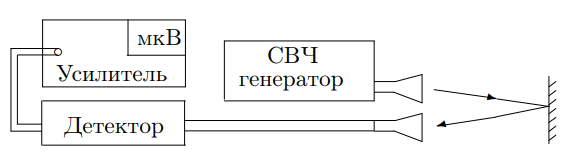
\includegraphics[width=1\linewidth]{fig1.PNG}
\caption{Схема опыта Франка и Герца} %% подпись к рисунку
\label{ris:experimoriginal} %% метка рисунка для ссылки на него
\end{minipage}
\hfill 
\begin{minipage}[h]{0.45\linewidth}
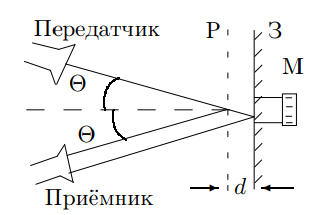
\includegraphics[width=1\linewidth]{fig2.PNG}
\caption{Схематический вид зависимости тока коллектора от напряжения на аноде}
\label{ris:experimcoded}
\end{minipage}
\end{center}
\end{figure}

Объясним вид зависимости тока коллектора (измеряется микроамперметром) от напряжения на аноде. При увеличении потенциала анода ток в лампе сначала растёт (зависимость, подобная ВАХ вакуумного диода). Когда энергия электронов становится достаточной для возбуждения атомов, ток коллектора резко уменьшается. Это происходит потому, что при неупругих соударениях с атомами электроны теряют свою энергию и не могут преодолеть задерживающее напряжение (около 1 В) между анодом и коллектором. При дальнейшем увеличении потенциала ток коллектора вновь возрастает: электроны, испытавшие неупругие соударения, при дальнейшем движении к аноду успевают набрать энергию, достаточную для преодоления задерживающего потенциала. Следующее замедление роста тока происходит в момент, когда часть электронов неупруго сталкивается с атомами два раза. Таким образом, на кривой зависимости тока коллектора от напряжения анода имеется ряд максимумов и минимумов, отстоящих друг от друга на равные расстояния, равные энергии первого возбуждённого состояния.

\section{Методика измерений}

\begin{figure}[h]
    \centering
    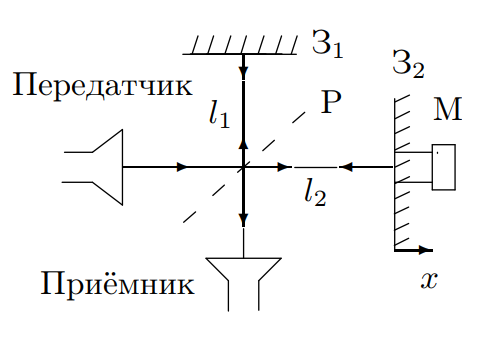
\includegraphics[width=12cm]{fig3.PNG}
    \caption{Схема экспериментальной установки}
    \label{fig:vac}
\end{figure}

На рис.~\ref{fig:vac} обозначены:
\begin{itemize}
    \item А --- амперметр
    \item Б7-4 --- стабилизированный источник питания (подаёт напряжение накала)
    \item $K_1$ --- тумблер для включения в цепь источника Б7-4
    \item Б5-10 --- выпрямитель (подаёт на анод ускоряющее напряжение)
    \item $Pi_3$ --- потенциометр, регулирующий величину ускоряющего напряжения
    \item $V_1$ --- вольтметр, измеряющий величину ускоряющего напряжения
    \item 4,5 В --- батарея КБСЛ --- источник задерживающего потенциала
    \item $Pi_2$ --- потенциометр, регулирующий величину задерживающего потенциала
    \item $V_2$ --- вольтметр, измеряющий величину задерживающего потенциала
    \item $\mu A$ --- микроамперметр --- регистрирует ток в цепи коллектора
    \item $K_3$ --- ключ, переключающий схему из статического режима в динамический
    \item Т --- понижающий трансформатор --- подаёт ускоряющий потенциал при динамическом режиме
    \item R --- нагрузочный резистор
\end{itemize}

\begin{figure}[h!]
\begin{center}
    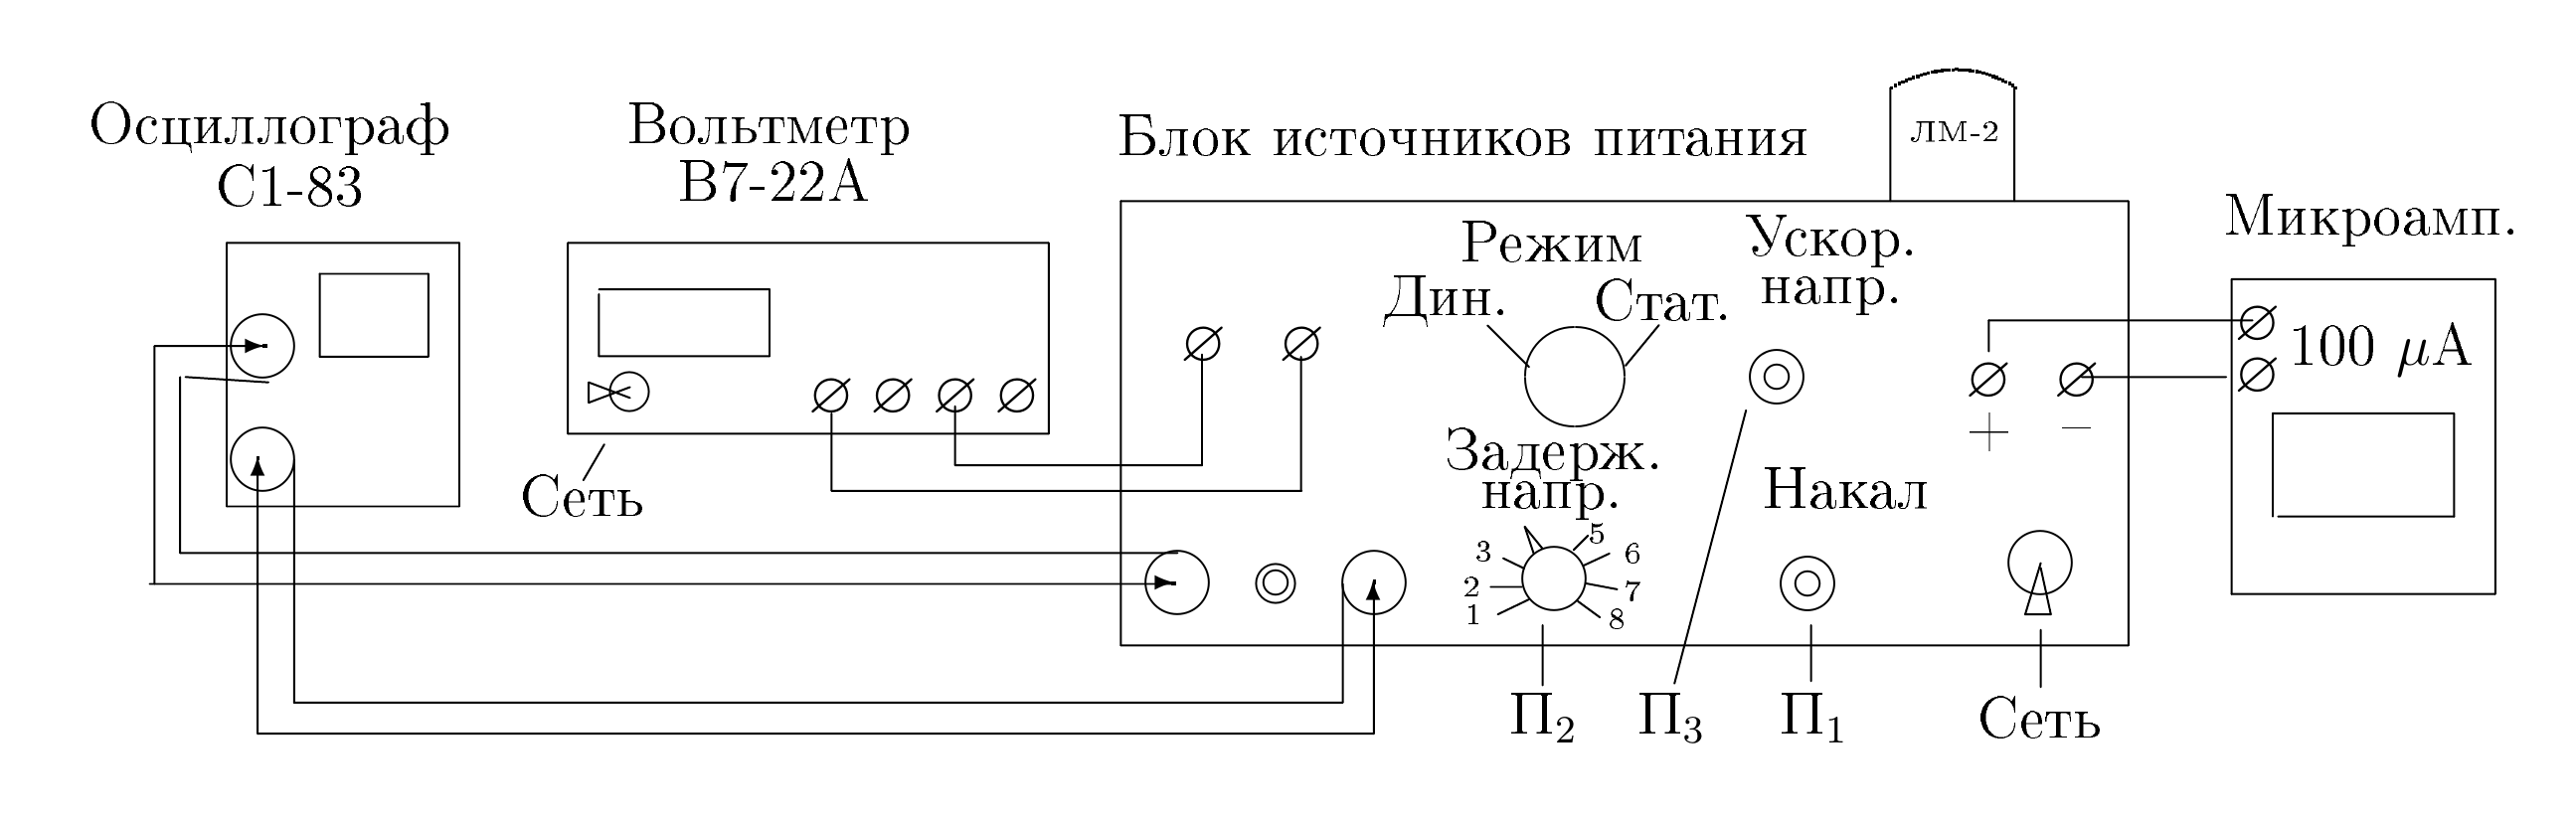
\includegraphics[width=\linewidth]{fig4.png}
\end{center}
\caption{Блок-схема экспериментальной установки}
\label{fig:ust}
\end{figure}

\section{Используемое оборудование}

\begin{enumerate}
    \item вольтметр;
    \item блок питания;
    \item микроамперметр;
    \item лампа ионизационного манометра ЛМ-2;
    \item осциллограф;
\end{enumerate}

\section{Результаты измерений и обработка данных}

\subsection{Динамический режим}

Осциллограмма ВАХ при измерении в динамическом режиме при различных значениях задерживающего напряжения представлена на рис.~\ref{fig:osc}.

\begin{figure}[h]
		\begin{minipage}[h]{0.3\linewidth}			\center{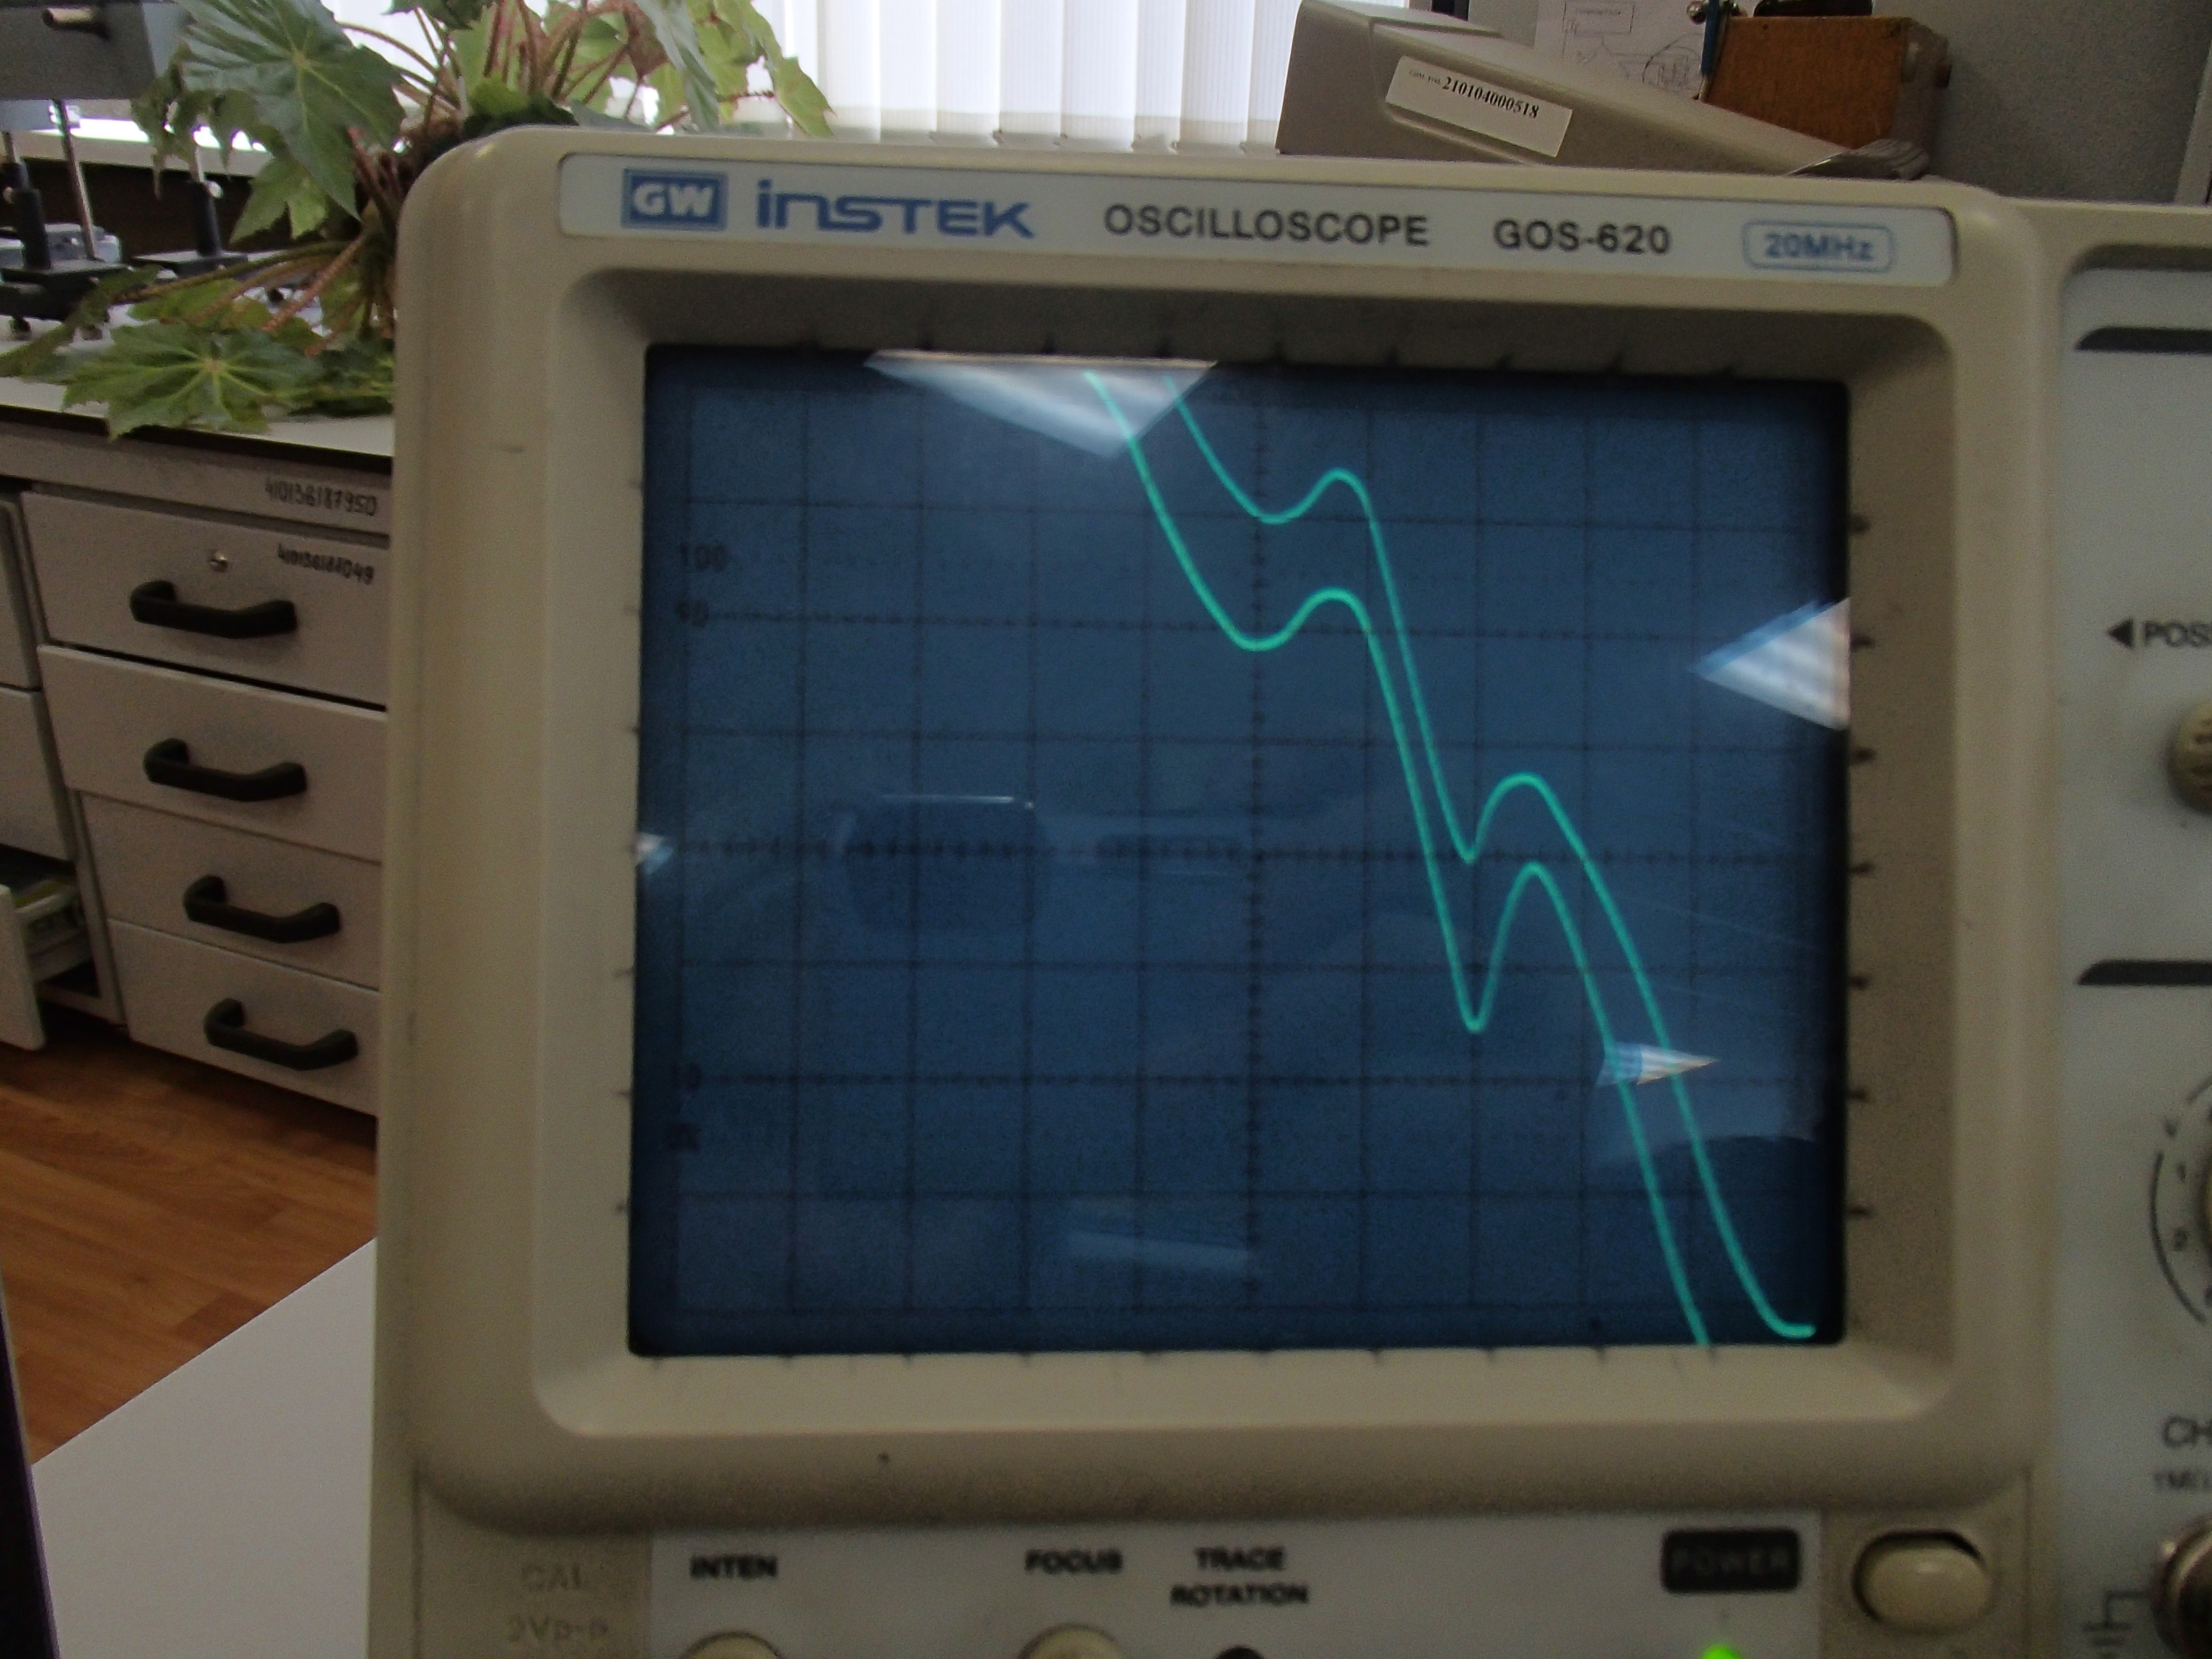
\includegraphics[width=0.9\linewidth]{osc1.jpg} \\ a)}
		\end{minipage}
		\hfill
		\begin{minipage}[h]{0.3\linewidth}
			\center{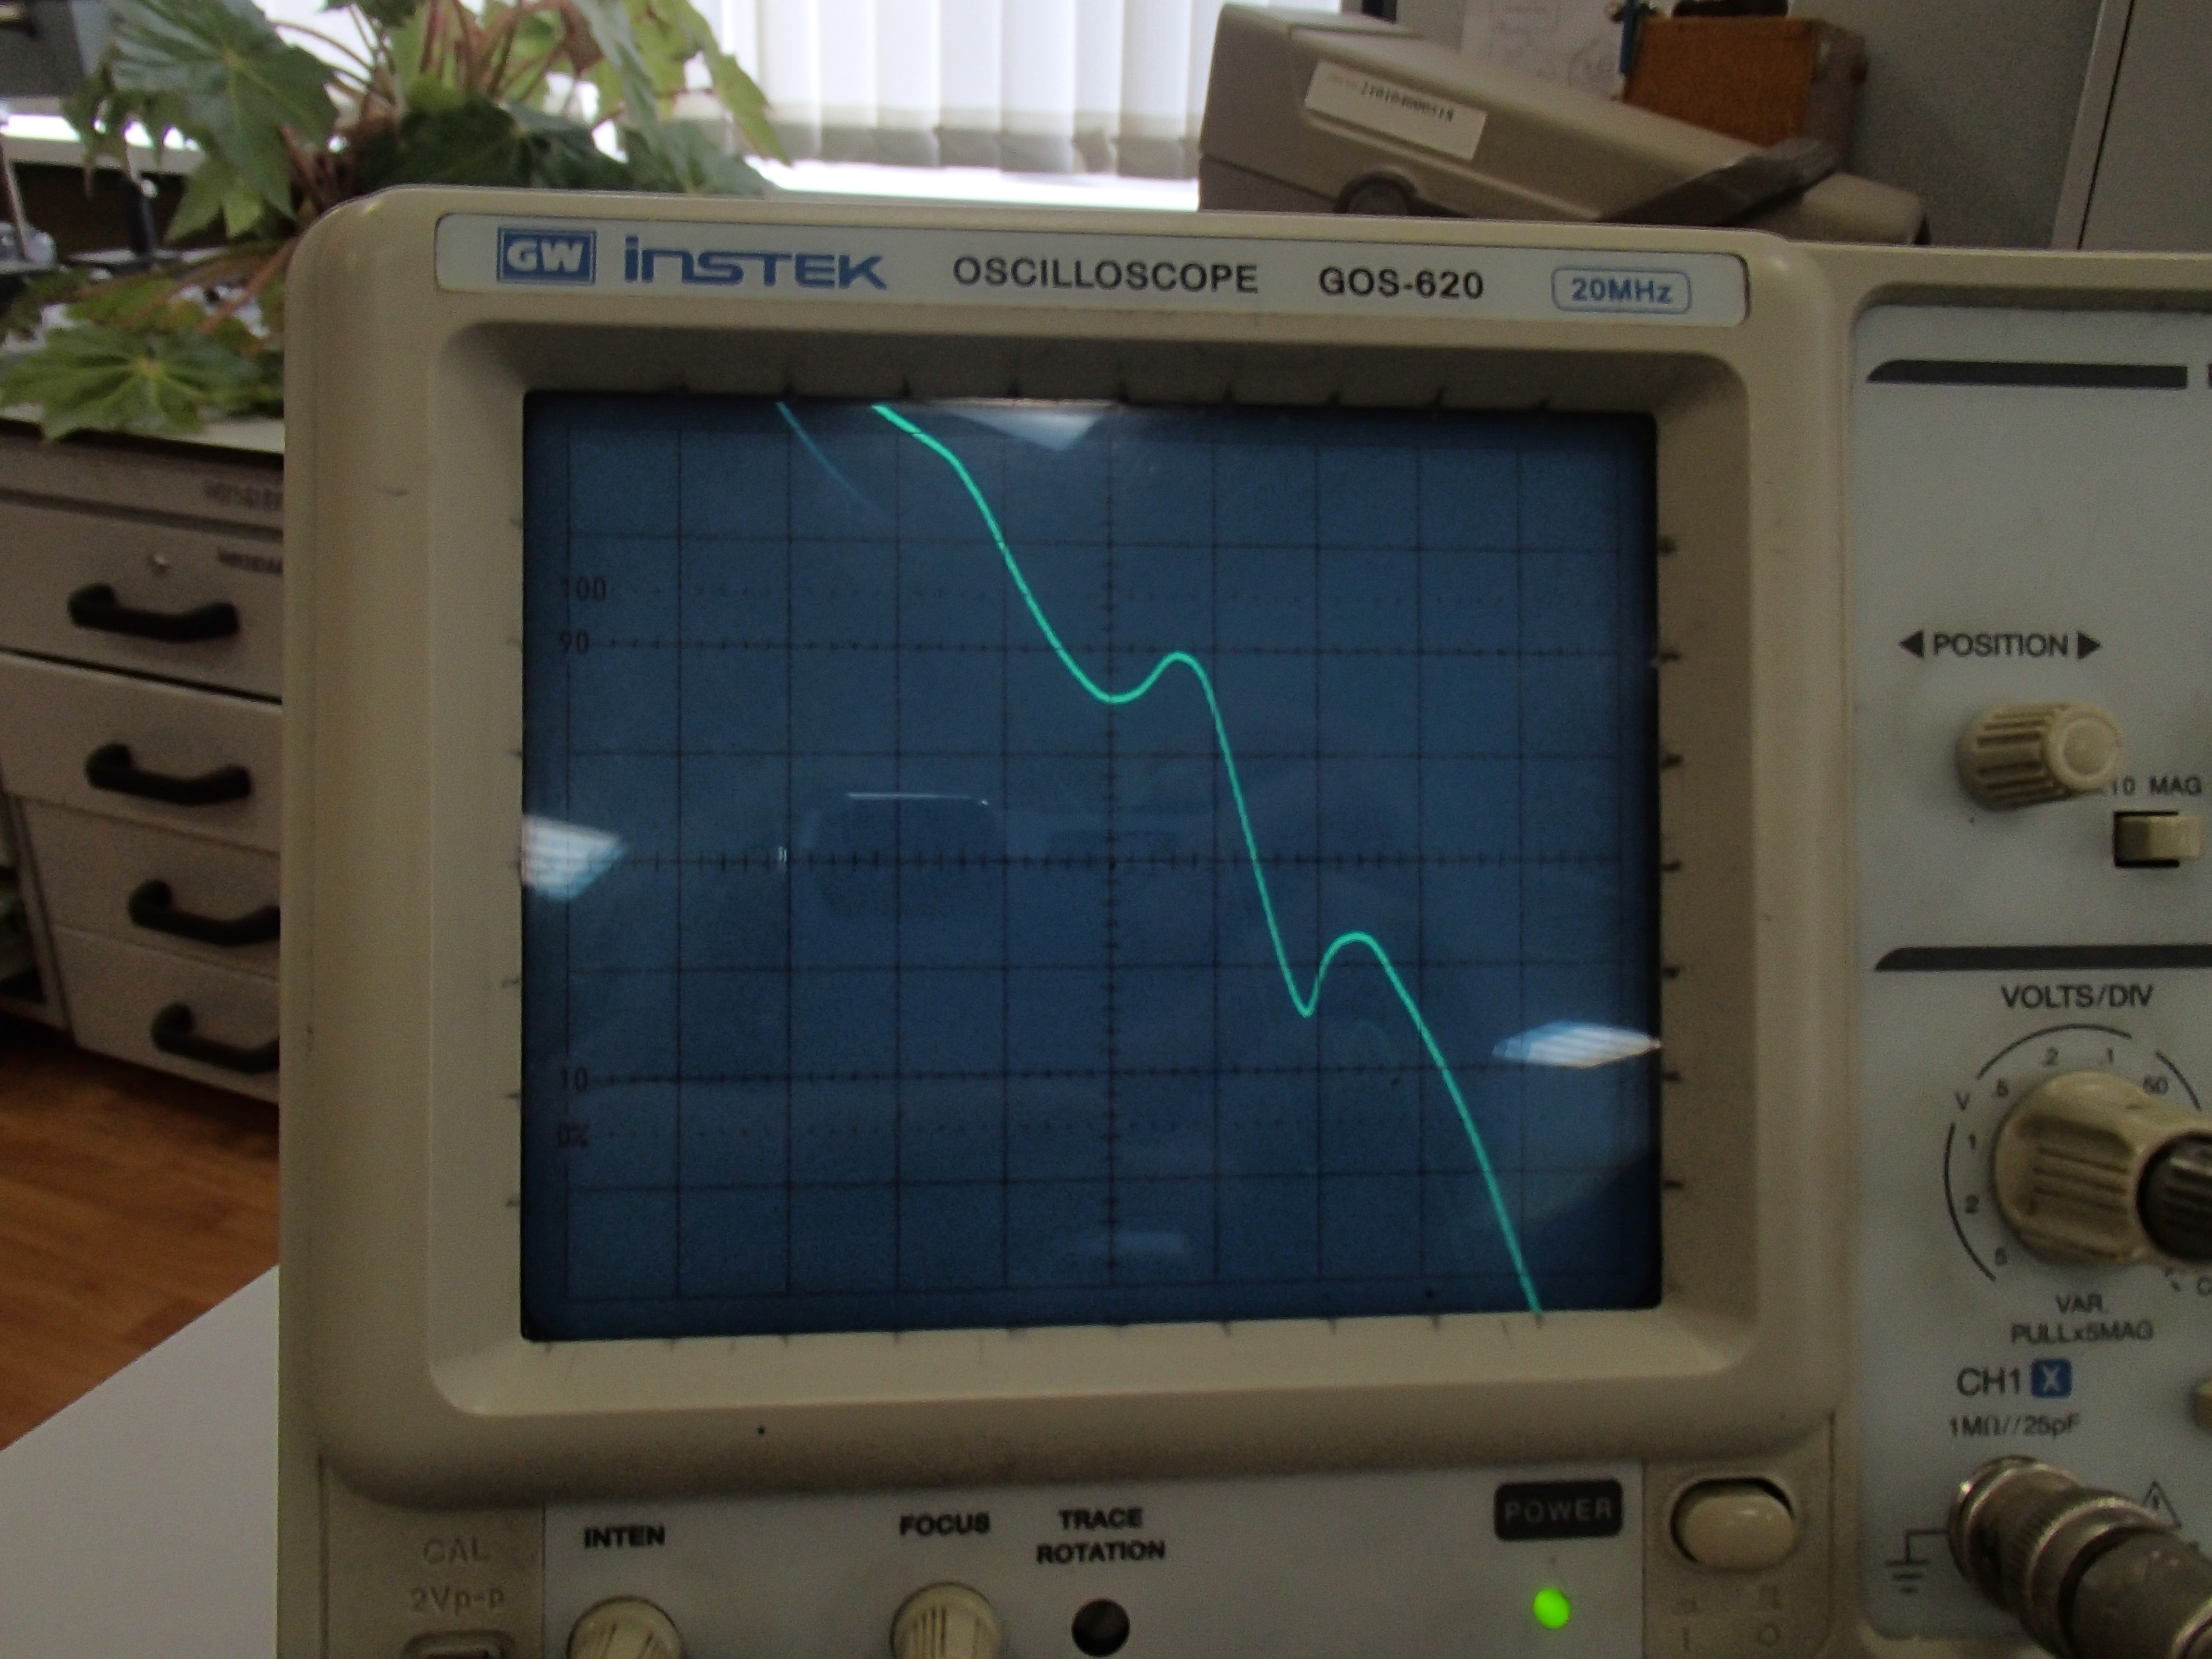
\includegraphics[width=0.9\linewidth]{osc2.jpg} \\ b)}
		\end{minipage}
		\hfill
		\begin{minipage}[h]{0.3\linewidth}
			\center{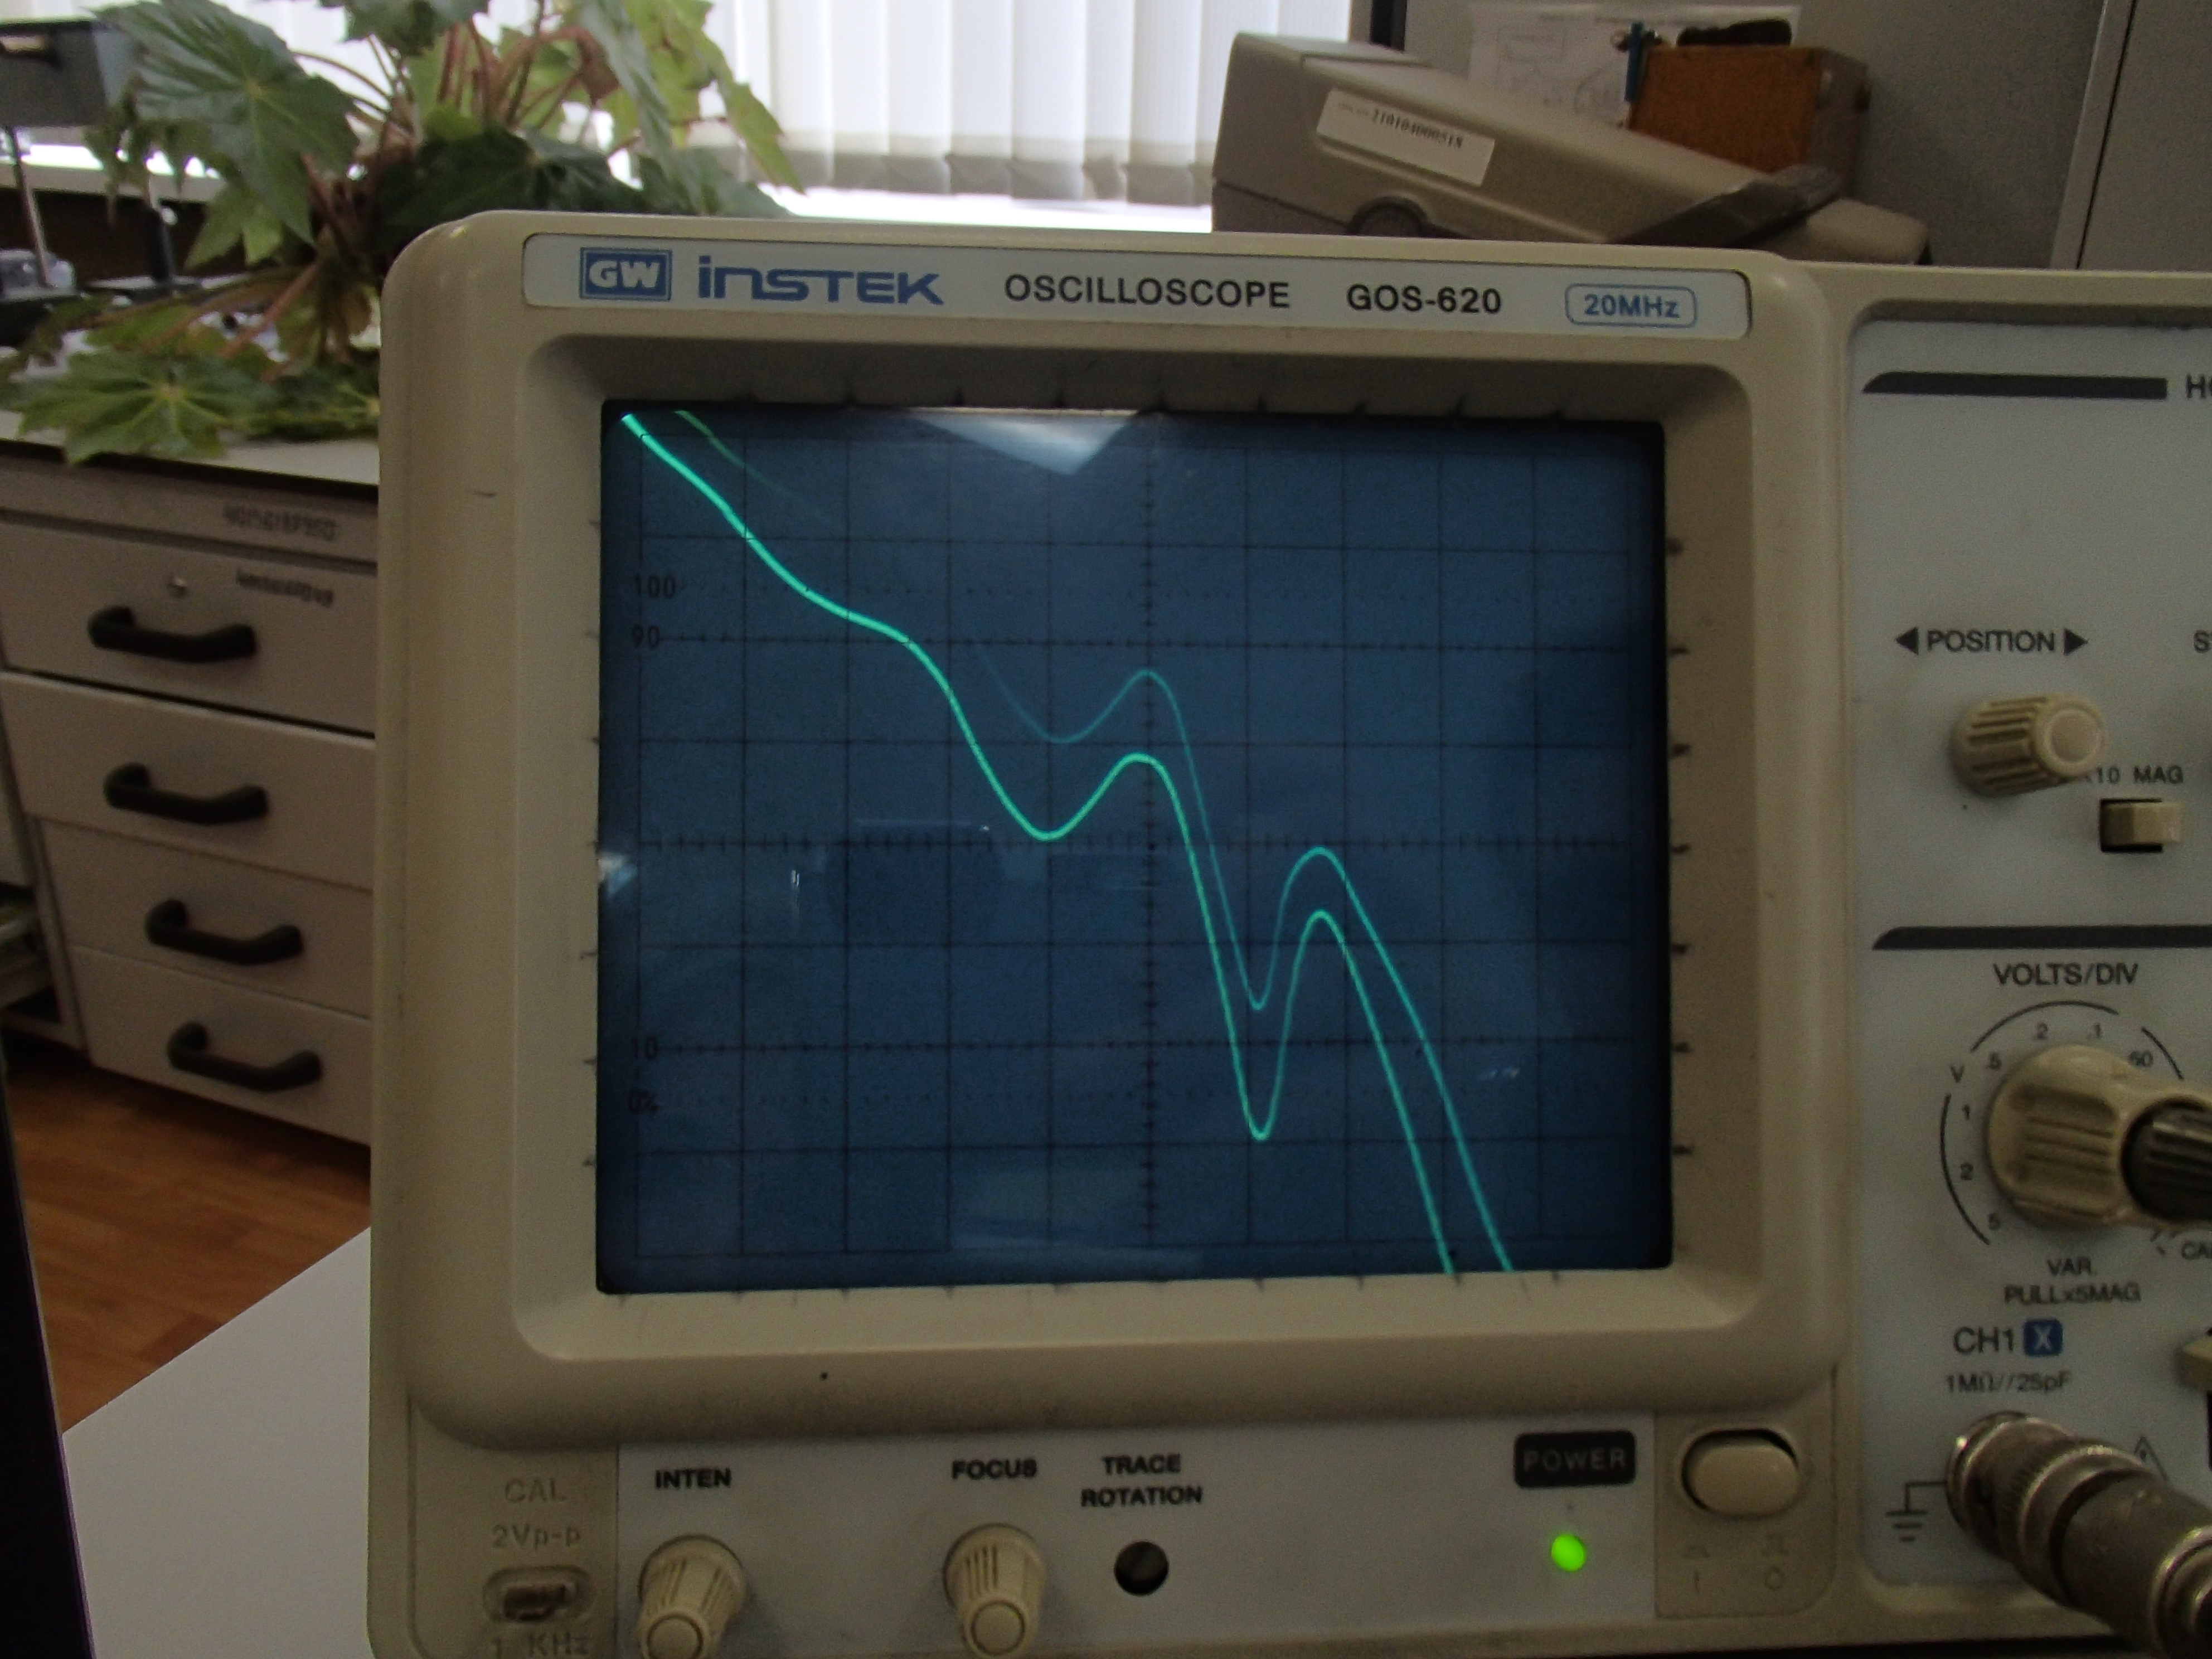
\includegraphics[width=0.9\linewidth]{osc3.jpg} \\ c)}
		\end{minipage}
		\caption{Осциллограммы: (a) $V = 4~B$, (b) $V = 6~B$, (c) $V = 8~B$}
		\label{fig:osc}
\end{figure}

По осциллограмме определим расстояние между максимумами и минимумами:

\begin{table}[h!]
\begin{center}
\begin{tabular}{|c|c|c|}
\hline 
Задерживающие напряжение & $\Delta{V_{max}}$, В & $\Delta{V_{min}}$, В \\ 
\hline 
4 В & $18,0\pm0,5$ & $20,0\pm0,5$ \\ 
\hline 
6 В & $18,0\pm0,5$ & $22,0\pm0,5$ \\ 
\hline 
8 В & $18,0\pm0,5$ & $22,0\pm0,5$ \\ 
\hline 
\end{tabular} 
\end{center}
\caption{Полученные значения в динамическом режиме измерений}
\label{tab:dyn}
\end{table}

Таким образом, энергия возбуждения первого уровня атома гелия $E = 18,0\pm1,2~эВ$.

\subsection{Статический режим}

Полученные данные в статическом режиме измерений представлены в таб.~\ref{tab:static}. По этим данным построим график на рис.~\ref{fig:plot}.

\begin{table}[h!]
\begin{center}
\begin{tabular}{|cccccc|}
\hline
\multicolumn{6}{|c|}{{ Задерживающее напряжение}}                                                                                                                                                                                                                                 \\ \hline
\multicolumn{2}{|c|}{{ 4 В}}                                                           & \multicolumn{2}{c|}{{ 6 В}}                                                          & \multicolumn{2}{c|}{{ 8 В}}                                     \\ \hline
\multicolumn{1}{|c|}{{ $V_a$, В}}  & \multicolumn{1}{c|}{{ mA}}      & \multicolumn{1}{c|}{{ $V_a$, В}}    & \multicolumn{1}{c|}{{ mA}}     & \multicolumn{1}{c|}{{ $V_a$, В}}    & { mA}     \\ \hline
\multicolumn{1}{|c|}{{ 0,04}}  & \multicolumn{1}{c|}{{ 0,0115}}  & \multicolumn{1}{c|}{{ 0,04}}  & \multicolumn{1}{c|}{{ 0,0069}} & \multicolumn{1}{c|}{{ 0,03}}  & { 0,007}  \\ \hline
\multicolumn{1}{|c|}{{ 4,42}}  & \multicolumn{1}{c|}{{ 0,0617}}  & \multicolumn{1}{c|}{{ 3,53}}  & \multicolumn{1}{c|}{{ 0,0296}} & \multicolumn{1}{c|}{{ 3,89}}  & { 0,0117} \\ \hline
\multicolumn{1}{|c|}{{ 9,25}}  & \multicolumn{1}{c|}{{ 0,1388}}  & \multicolumn{1}{c|}{{ 7,62}}  & \multicolumn{1}{c|}{{ 0,0907}} & \multicolumn{1}{c|}{{ 8,58}}  & { 0,0772} \\ \hline
\multicolumn{1}{|c|}{{ 13,57}} & \multicolumn{1}{c|}{{ 0,2}}     & \multicolumn{1}{c|}{{ 11,06}} & \multicolumn{1}{c|}{{ 0,1481}} & \multicolumn{1}{c|}{{ 16,06}} & { 0,1963} \\ \hline
\multicolumn{1}{|c|}{{ 16,62}} & \multicolumn{1}{c|}{{ 0,2363}}  & \multicolumn{1}{c|}{{ 13,76}} & \multicolumn{1}{c|}{{ 0,1895}} & \multicolumn{1}{c|}{{ 21,49}} & { 0,2463} \\ \hline
\multicolumn{1}{|c|}{{ 20,09}} & \multicolumn{1}{c|}{{ 0,2605}}  & \multicolumn{1}{c|}{{ 21,89}} & \multicolumn{1}{c|}{{ 0,2551}} & \multicolumn{1}{c|}{{ 23,25}} & { 0,1974} \\ \hline
\multicolumn{1}{|c|}{{ 22,25}} & \multicolumn{1}{c|}{{ 0,2589}}  & \multicolumn{1}{c|}{{ 23,3}}  & \multicolumn{1}{c|}{{ 0,194}}  & \multicolumn{1}{c|}{{ 25,32}} & { 0,0926} \\ \hline
\multicolumn{1}{|c|}{{ 24,03}} & \multicolumn{1}{c|}{{ 0,1965}}  & \multicolumn{1}{c|}{{ 25,08}} & \multicolumn{1}{c|}{{ 0,1409}} & \multicolumn{1}{c|}{{ 27,02}} & { 0,087}  \\ \hline
\multicolumn{1}{|c|}{{ 26,08}} & \multicolumn{1}{c|}{{ 0,239}}   & \multicolumn{1}{c|}{{ 26,3}}  & \multicolumn{1}{c|}{{ 0,1372}} & \multicolumn{1}{c|}{{ 28,71}} & { 0,1132} \\ \hline
\multicolumn{1}{|c|}{{ 28,54}} & \multicolumn{1}{c|}{{ 0,2713}}  & \multicolumn{1}{c|}{{ 27,02}} & \multicolumn{1}{c|}{{ 0,1722}} & \multicolumn{1}{c|}{{ 30,04}} & { 0,1601} \\ \hline
\multicolumn{1}{|c|}{{ 33,71}} & \multicolumn{1}{c|}{{ 0,362}}   & \multicolumn{1}{c|}{{ 31,1}}  & \multicolumn{1}{c|}{{ 0,2588}} & \multicolumn{1}{c|}{{ 34,65}} & { 0,2563} \\ \hline
\multicolumn{1}{|c|}{{ 38,74}} & \multicolumn{1}{c|}{{ 0,38967}} & \multicolumn{1}{c|}{{ 33,74}} & \multicolumn{1}{c|}{{ 0,3095}} & \multicolumn{1}{c|}{{ 38,93}} & { 0,2857} \\ \hline
\multicolumn{1}{|c|}{{ 40,57}} & \multicolumn{1}{c|}{{ 0,3857}}  & \multicolumn{1}{c|}{{ 39,8}}  & \multicolumn{1}{c|}{{ 0,3403}} & \multicolumn{1}{c|}{{ 48,31}} & { 0,2269} \\ \hline
\multicolumn{1}{|c|}{{ 42,4}}  & \multicolumn{1}{c|}{{ 0,3682}}  & \multicolumn{1}{c|}{{ 45,4}}  & \multicolumn{1}{c|}{{ 0,3045}} & \multicolumn{1}{c|}{{ 55,75}} & { 0,2674} \\ \hline
\multicolumn{1}{|c|}{{ 44,99}} & \multicolumn{1}{c|}{{ 0,3786}}  & \multicolumn{1}{c|}{{ 50,34}} & \multicolumn{1}{c|}{{ 0,3195}} & \multicolumn{1}{c|}{{ 64,47}} & { 0,3064} \\ \hline
\multicolumn{1}{|c|}{{ 48,58}} & \multicolumn{1}{c|}{{ 0,3885}}  & \multicolumn{1}{c|}{{ 56,25}} & \multicolumn{1}{c|}{{ 0,3688}} & \multicolumn{1}{c|}{{ 76,95}} & { 0,3181} \\ \hline
\multicolumn{1}{|c|}{{ 54,22}} & \multicolumn{1}{c|}{{ 0,4363}}  & \multicolumn{1}{c|}{{ 61,83}} & \multicolumn{1}{c|}{{ 0,401}}  & \multicolumn{1}{c|}{{ 50,92}} & { 0,213}  \\ \hline
\multicolumn{1}{|c|}{{ 62,27}} & \multicolumn{1}{c|}{{ 0,495}}   & \multicolumn{1}{c|}{{ 70,85}} & \multicolumn{1}{c|}{{ 0,417}}  & \multicolumn{1}{c|}{{ 46,37}} & { 0,209}  \\ \hline
\multicolumn{1}{|c|}{{ 67,84}} & \multicolumn{1}{c|}{{ 0,5108}}  & \multicolumn{1}{c|}{{ 76,77}} & \multicolumn{1}{c|}{{ 0,4387}} & \multicolumn{1}{c|}{{ }}      & { }       \\ \hline
\multicolumn{1}{|c|}{{ 76,05}} & \multicolumn{1}{c|}{{ 0,5591}}  & \multicolumn{1}{c|}{{ 43,42}} & \multicolumn{1}{c|}{{ 0,2722}} & \multicolumn{1}{c|}{{ }}      & { }       \\ \hline
\multicolumn{1}{|c|}{{ }}      & \multicolumn{1}{c|}{{ }}        & \multicolumn{1}{c|}{{ 47,23}} & \multicolumn{1}{c|}{{ 0,2672}} & \multicolumn{1}{c|}{{ }}      & { }       \\ \hline
\end{tabular}
\end{center}
\caption{Полученные значения в статическом режиме измерений}
\label{tab:static}
\end{table}

\begin{figure}[h!]
\begin{center}
    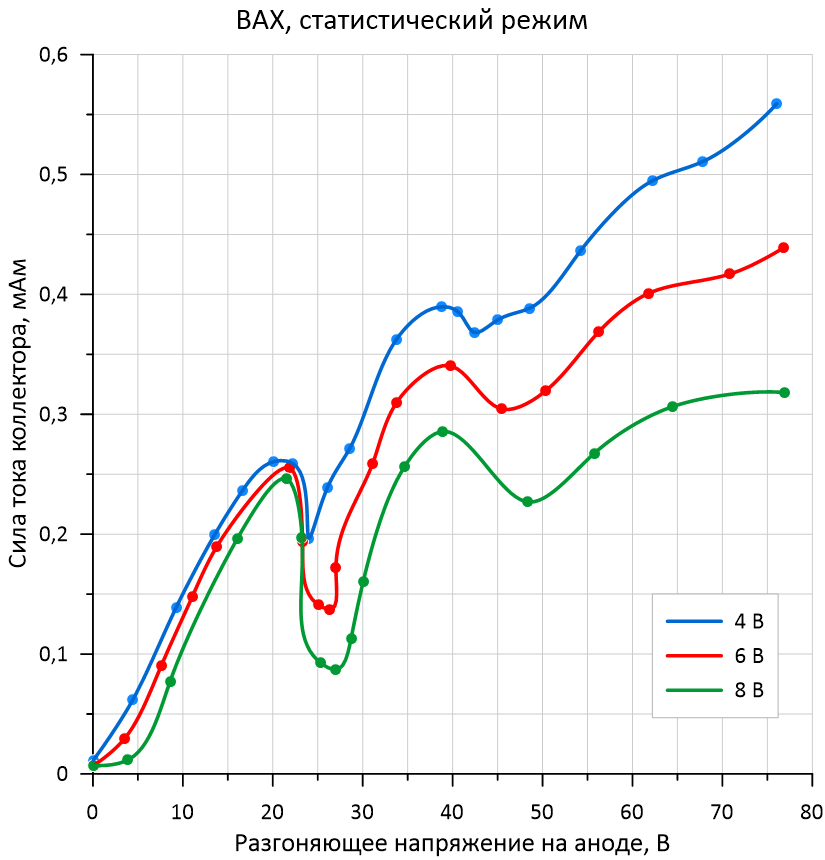
\includegraphics[width=0.7\linewidth]{2_1.png}
\end{center}
\caption{Вольт-амперная характеристика лампы}
\label{fig:plot}
\end{figure}

По графику (рис.~\ref{fig:plot}) определим расстояние между максимумами и минимумами ВАХ.

\begin{table}[h!]
\begin{center}
\begin{tabular}{|c|c|c|}
\hline 
Задерживающие напряжение & $\Delta{V_{max}}$, В & $\Delta{V_{min}}$, В \\ 
\hline 
4 В & $18,0\pm2,5$ & $18,0\pm2,5$ \\ 
\hline 
6 В & $18,0\pm2,5$ & $19,0\pm2,5$ \\ 
\hline 
8 В & $17,0\pm2,5$ & $20,0\pm2,5$ \\ 
\hline 
\end{tabular} 
\end{center}
\caption{Полученные значения в статическом режиме измерений}
\label{tab:stat}
\end{table}

Тогда получаем значение энергии $E = 17,5\pm2,7~эВ$.

\newpage

\section{Обсуждение результатов и выводы}

В ходе работы был воспроизведён опыт Франка-Герца, подтверждающий наличие дискретных уровней возбуждения атомов. Вольт-амперная характеристика трёхэлектродной вакуумной лампы была измерена двумя способами --- динамическим и статическим. По этим ВАХ были экспериментально определены потенциалы возбуждения атомов гелия (одноатомный газ, заполняющий лампу). Полученные значения:
$$ \boxed{E_{дин} = 18,0\pm1,2~эВ; \quad E_{стат} = 17,5\pm2,7~эВ} $$
Табличное значение для данной величины --- $E = 21,6~эВ$. Полученные результаты совпадают по порядку величины, также значение потенциала возбуждения атома гелия в пределах погрешности совпадает с табличным значением. Статический метод оказался менее точным, чем динамический, так как по конечному набору точек сложнее определить экстремумы.

\end{document}
